\documentclass{beamer}
% Essential packages
\usepackage{amsmath, mathtools}
\usepackage{graphicx}
\usepackage{ulem}
\usepackage{tikz}
\usetikzlibrary{shapes.geometric, arrows.meta, positioning, calc}
% Define custom TikZ styles for reuse
\tikzset{
  % Main diagram ring segments
  archsegment/.style={fill=blue!20, draw=black!70},
  archsegmentselected/.style={fill=blue!80, draw=black!90, text=white},
  % Tool nodes
  toolnode/.style={align=center, font=\tiny},
  % Path flow nodes
  pathnode/.style={draw, rounded corners, align=center, inner sep=5pt, font=\small},
  tool/.style={pathnode, fill=gray!10},
  file/.style={pathnode, fill=white},
  % Pointers
  calloutpointer/.style={->, line width=1pt, draw=black!80},
  flowpointer/.style={->, line width=1.2pt, draw=black!90},
}

% Theme selection
\usetheme{Madrid}
\usecolortheme{whale}

% Document metadata
\title{A Numerical Approach to Calculus}
\subtitle{Implementation of Taylor Series with Java and Python}
\author{Jaehoon Song}
\date{\today}

% Alternative metadata (commented out):
% \title{Integrating Runtimes into Operating Systems}
% \subtitle{Abstraction, Environment, and Computation Workflow}

\begin{document}

% Title slide
\begin{frame}
  \titlepage
\end{frame}

% Section 1: Introduction
\begin{frame}{Introduction}
  \begin{itemize}
    \item \textbf{Programming fundamentals:} We start with how \textbf{abstraction} and the \textbf{operating system} stack (OS, shell, runtimes like the JVM and Python) hide hardware details and make development tractable.
    \item \textbf{Mathematical abstraction:} We then study the \textbf{Taylor series}---another abstraction: replacing a function with an (in principle infinite) polynomial built from derivatives and powers of $x$.
    \item \textbf{Irrational values in practice:} Machines do not store exact irrationals; they use \textbf{finite} floating-point words and \textbf{truncated} series so values are represented as well-chosen approximations, not infinite decimals.
    \item \textbf{Finite logic vs.\ infinite theory:} Computer programs run for finitely many steps at fixed precision, yet they can still embody ``infinite'' calculus ideas by stopping after enough terms and living inside tolerances and error bounds.
  \end{itemize}
\end{frame}

% Slide 2: Abstraction: A Multi-Level Stack
\begin{frame}{Abstraction}
  \begin{itemize}
    \item \textbf{Abstraction:} Hiding complex details behind a simpler interface. (\uline{You don't need to know how it works, just what it does.})
    \item \textbf{OS Abstraction:} abstraction of hardware resource management and system calls.
    \item \textbf{Shell Abstraction:} command-line interface, abstraction of interacting with the OS and executing utilities.
    \item \textbf{Runtime Abstraction (JDK/Python):} abstraction of machines, running code on a virtual machine (JVM) or interpreter.
  \end{itemize}
  \vspace{0.3cm}
  \begin{footnotesize}
    \textbf{Script Automation:} abstraction of environment setup; \texttt{dev.bat} / \texttt{dev.sh} will be provided to quickly set up your environment for these layers.
  \end{footnotesize}
  \vspace{0.3cm}
  \begin{alertblock}{Next Step}
    Let's give a quick overview of how the OS, Shell, JDK, and Python relate by visualizing their place in the system hierarchy.
  \end{alertblock}
\end{frame}

% Slide 3: OS layers and Java / Python runtime abstraction (external figure)
\begin{frame}{Operating System \& Language Abstraction}
  \begin{center}
    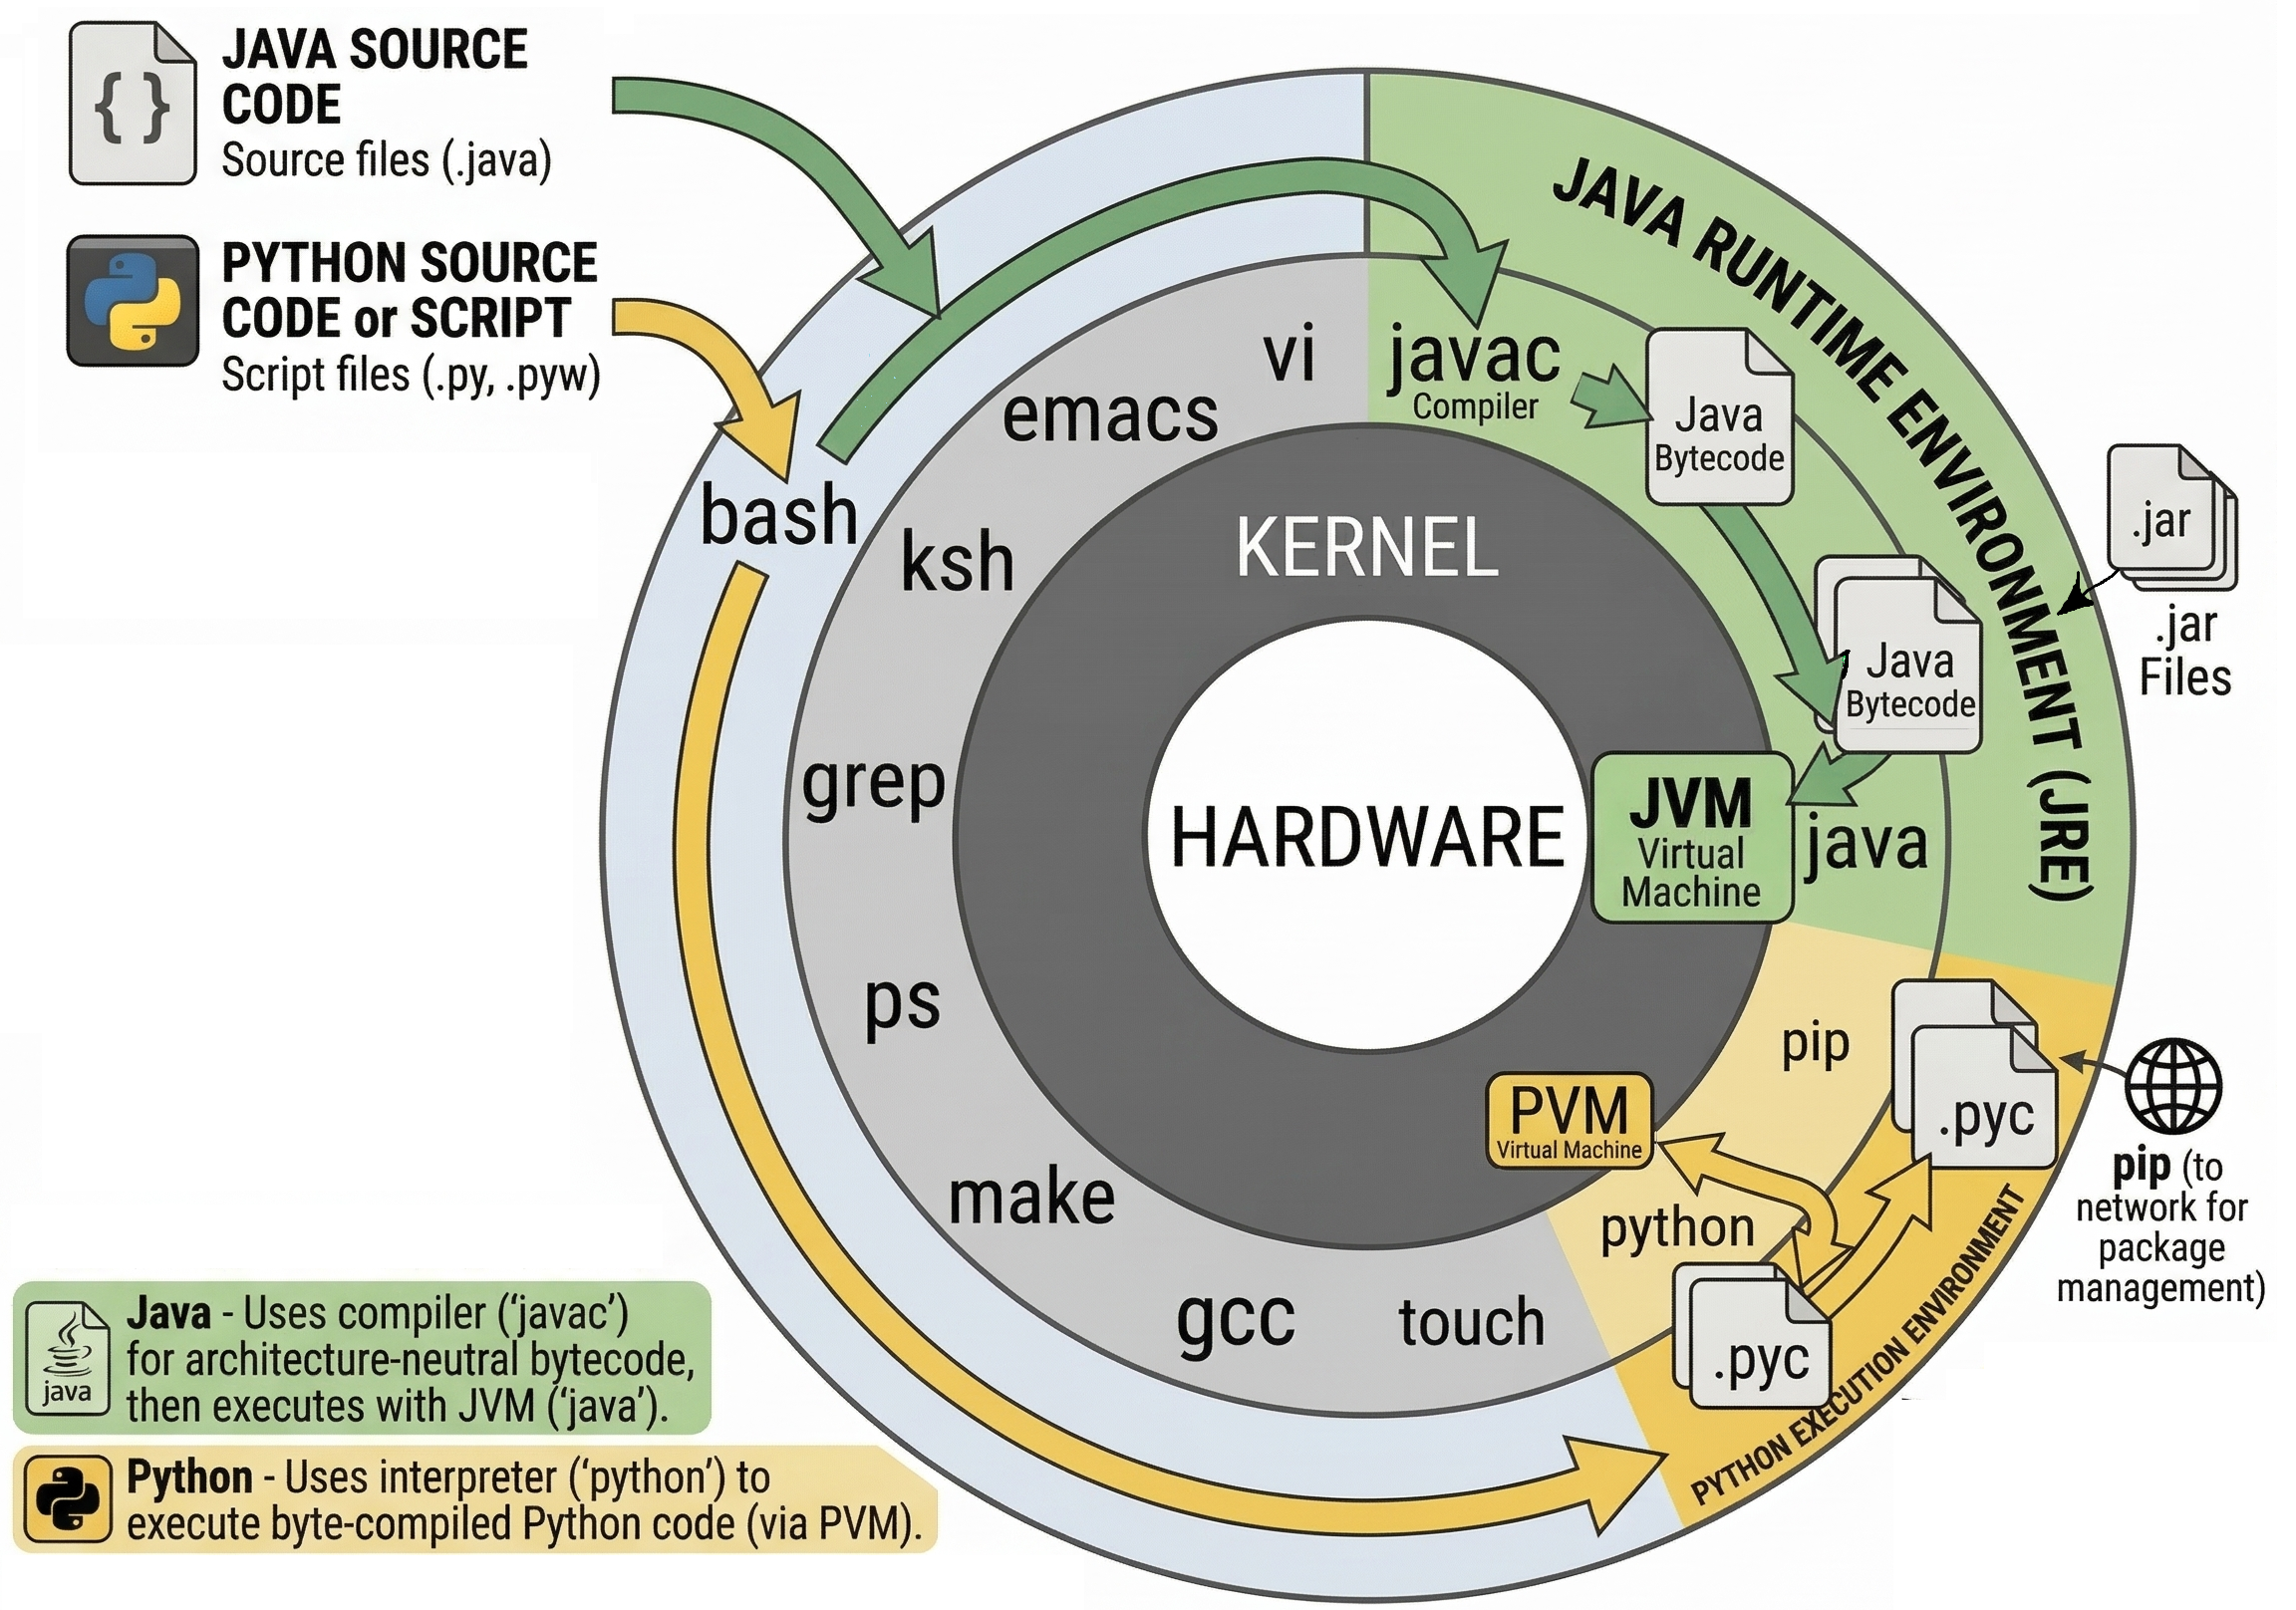
\includegraphics[width=0.98\linewidth,height=0.72\textheight,keepaspectratio]{images/os_and_lang_abstraction.png}
  \end{center}
\end{frame}

% Slide 4: Environment Setup & Tool Detection
\begin{frame}[fragile]{Environment Setup \& Detection}
  \begin{itemize}
    \item \textbf{Finding the Tools:} When a command is typed (\texttt{javac Main.java}), the shell searches the system \texttt{PATH} environment variable.
    \item \textbf{PATH Variable:} A semicolon- or colon-separated list of directories containing executables.
    \item \textbf{Example Detection Sequence:}
      \begin{enumerate}
        \item User types command.
        \item Shell looks in directories defined in \texttt{PATH}.
        \item First executable found is run (or error).
      \end{enumerate}
    \item \textbf{Automation via \texttt{dev.sh} / \texttt{dev.bat}:} Conceptually, these scripts modify the local session environment to automatically detect these tools.
  \end{itemize}
  \begin{block}{Conceptual \texttt{dev.sh} Snippet}
\begin{verbatim}
export JDK_HOME="/path/to/jdk-17"
export PYTHON_HOME="/path/to/python3.9"
export PATH="$JDK_HOME/bin:$PYTHON_HOME/bin:$PATH"
\end{verbatim}
  \end{block}
\end{frame}

% Slide 5: Java Compilation & Execution Workflow (Compilation Diagram)
\begin{frame}{Java: Compile-Once, Run-Everywhere}
  \begin{center}
    \resizebox{0.98\linewidth}{!}{%
    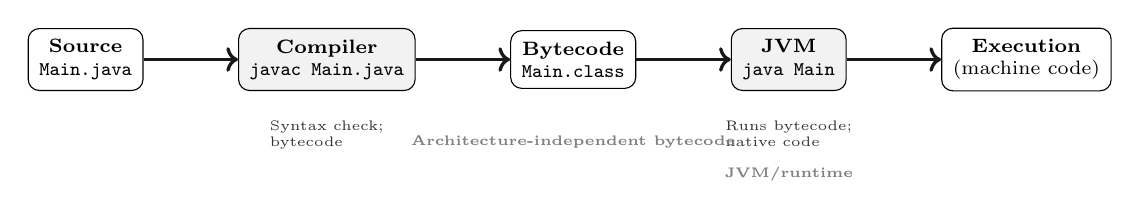
\begin{tikzpicture}[
      node distance=1.2cm,
      pathnode/.style={draw, rounded corners, align=center, inner sep=4pt, font=\scriptsize},
      tool/.style={pathnode, fill=gray!10},
      file/.style={pathnode, fill=white},
    ]

      % Define flow nodes
      \node[file] (source) {\textbf{Source} \\ \texttt{Main.java}};
      \node[tool, right=of source] (compiler) {\textbf{Compiler} \\ \texttt{javac Main.java}};
      \node[file, right=of compiler] (bytecode) {\textbf{Bytecode} \\ \texttt{Main.class}};
      \node[tool, right=of bytecode] (interpreter) {\textbf{JVM} \\ \texttt{java Main}};
      \node[file, right=of interpreter] (exec) {\textbf{Execution} \\ (machine code)};

      \draw[flowpointer] (source) -- (compiler);
      \draw[flowpointer] (compiler) -- (bytecode);
      \draw[flowpointer] (bytecode) -- (interpreter);
      \draw[flowpointer] (interpreter) -- (exec);

      \node[toolnode, text=black!80, below=0.25cm of compiler, align=left, font=\tiny] {Syntax check; \\ bytecode};
      \node[toolnode, text=black!80, below=0.25cm of interpreter, align=left, font=\tiny] {Runs bytecode; \\ native code};

      \node[font=\bfseries\tiny, text=black!50] at ($(compiler.east)!0.5!(interpreter.west)+(0, -1.05)$) {Architecture-independent bytecode};
      \node[font=\bfseries\tiny, text=black!50] at ($(interpreter.south)+(0, -1.05)$) {JVM/runtime};

    \end{tikzpicture}%
    }
  \end{center}
  \vspace{0.3cm}
  \begin{alertblock}{Java Compilation Workflow}
    The \texttt{Main.java} is first compiled into a platform-independent format (bytecode)
    and then run by the JVM (Java Virtual Machine), \textbf{abstracting away system differences}.
  \end{alertblock}
\end{frame}

% Slide 6: Python Execution Flow
\begin{frame}{Python: Interpreted \& Dynamic}
  \begin{center}
    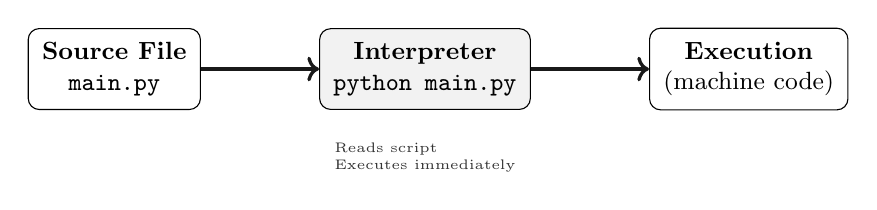
\begin{tikzpicture}[node distance=1.5cm, tool/.style={pathnode, fill=gray!10}, file/.style={pathnode, fill=white}]

      \node[file] (source) {\textbf{Source File} \\ \texttt{main.py}};
      \node[tool, right=of source] (interpreter) {\textbf{Interpreter} \\ \texttt{python main.py}};
      \node[file, right=of interpreter] (exec) {\textbf{Execution} \\ (machine code)};

      \draw[flowpointer] (source) -- (interpreter);
      \draw[flowpointer] (interpreter) -- (exec);

      \node[toolnode, text=black!80, below=0.3cm of interpreter, align=left] {Reads script \\ Executes immediately};

    \end{tikzpicture}
  \end{center}
  \vspace{0.3cm}
  \begin{alertblock}{Python Execution Workflow}
    The \texttt{main.py} is interpreted and executed line-by-line,
    which speeds up the write--test loop compared to a compile-then-run Java workflow,
    \textbf{abstracting away system differences}.
  \end{alertblock}
  \vspace{0.3cm}
  \begin{minipage}{0.96\linewidth}
    \footnotesize
    \textbf{Note:} Typical pure-Python code runs slower
    than comparable JVM bytecode (and usually slower than native code).
  \end{minipage}
\end{frame}

% Slide 7: The Computational Problem
\begin{frame}{Background: The Computational Problem}
  \begin{block}{Hardware Limitations}
    Digital circuits are inherently limited to basic arithmetic operations:
    \begin{itemize}
      \item Addition and Subtraction
      \item Multiplication and Division
    \end{itemize}
  \end{block}
  \vspace{0.5cm}
  Continuous functions, such as $\sin(x)$, cannot be stored as an infinite lookup table. Instead, these values must be approximated using iterative algorithms.
\end{frame}

% Slide 8: The Mathematical Theory
\begin{frame}{Abstraction: The Taylor Series Expansion}
  The $\sin(x)$ function can be represented as an infinite sum of powers:
  \begin{equation*}
    \sin(x) = \sum_{n=0}^{\infty} \frac{(-1)^n x^{2n+1}}{(2n+1)!} 
  \end{equation*}
  \vspace{0.3cm}
  This expansion is simplified into a sequence of polynomial terms:
  \begin{equation*}
    \sin(x) \approx x - \frac{x^3}{3!} + \frac{x^5}{5!} - \frac{x^7}{7!} + \dots
  \end{equation*}
  Higher accuracy is achieved as more terms are calculated.
\end{frame}

% Slide 9: Taylor Series of $\sin(x)$
\begin{frame}{Abstraction: Taylor Series of $\sin(x)$}
  \begin{center}
    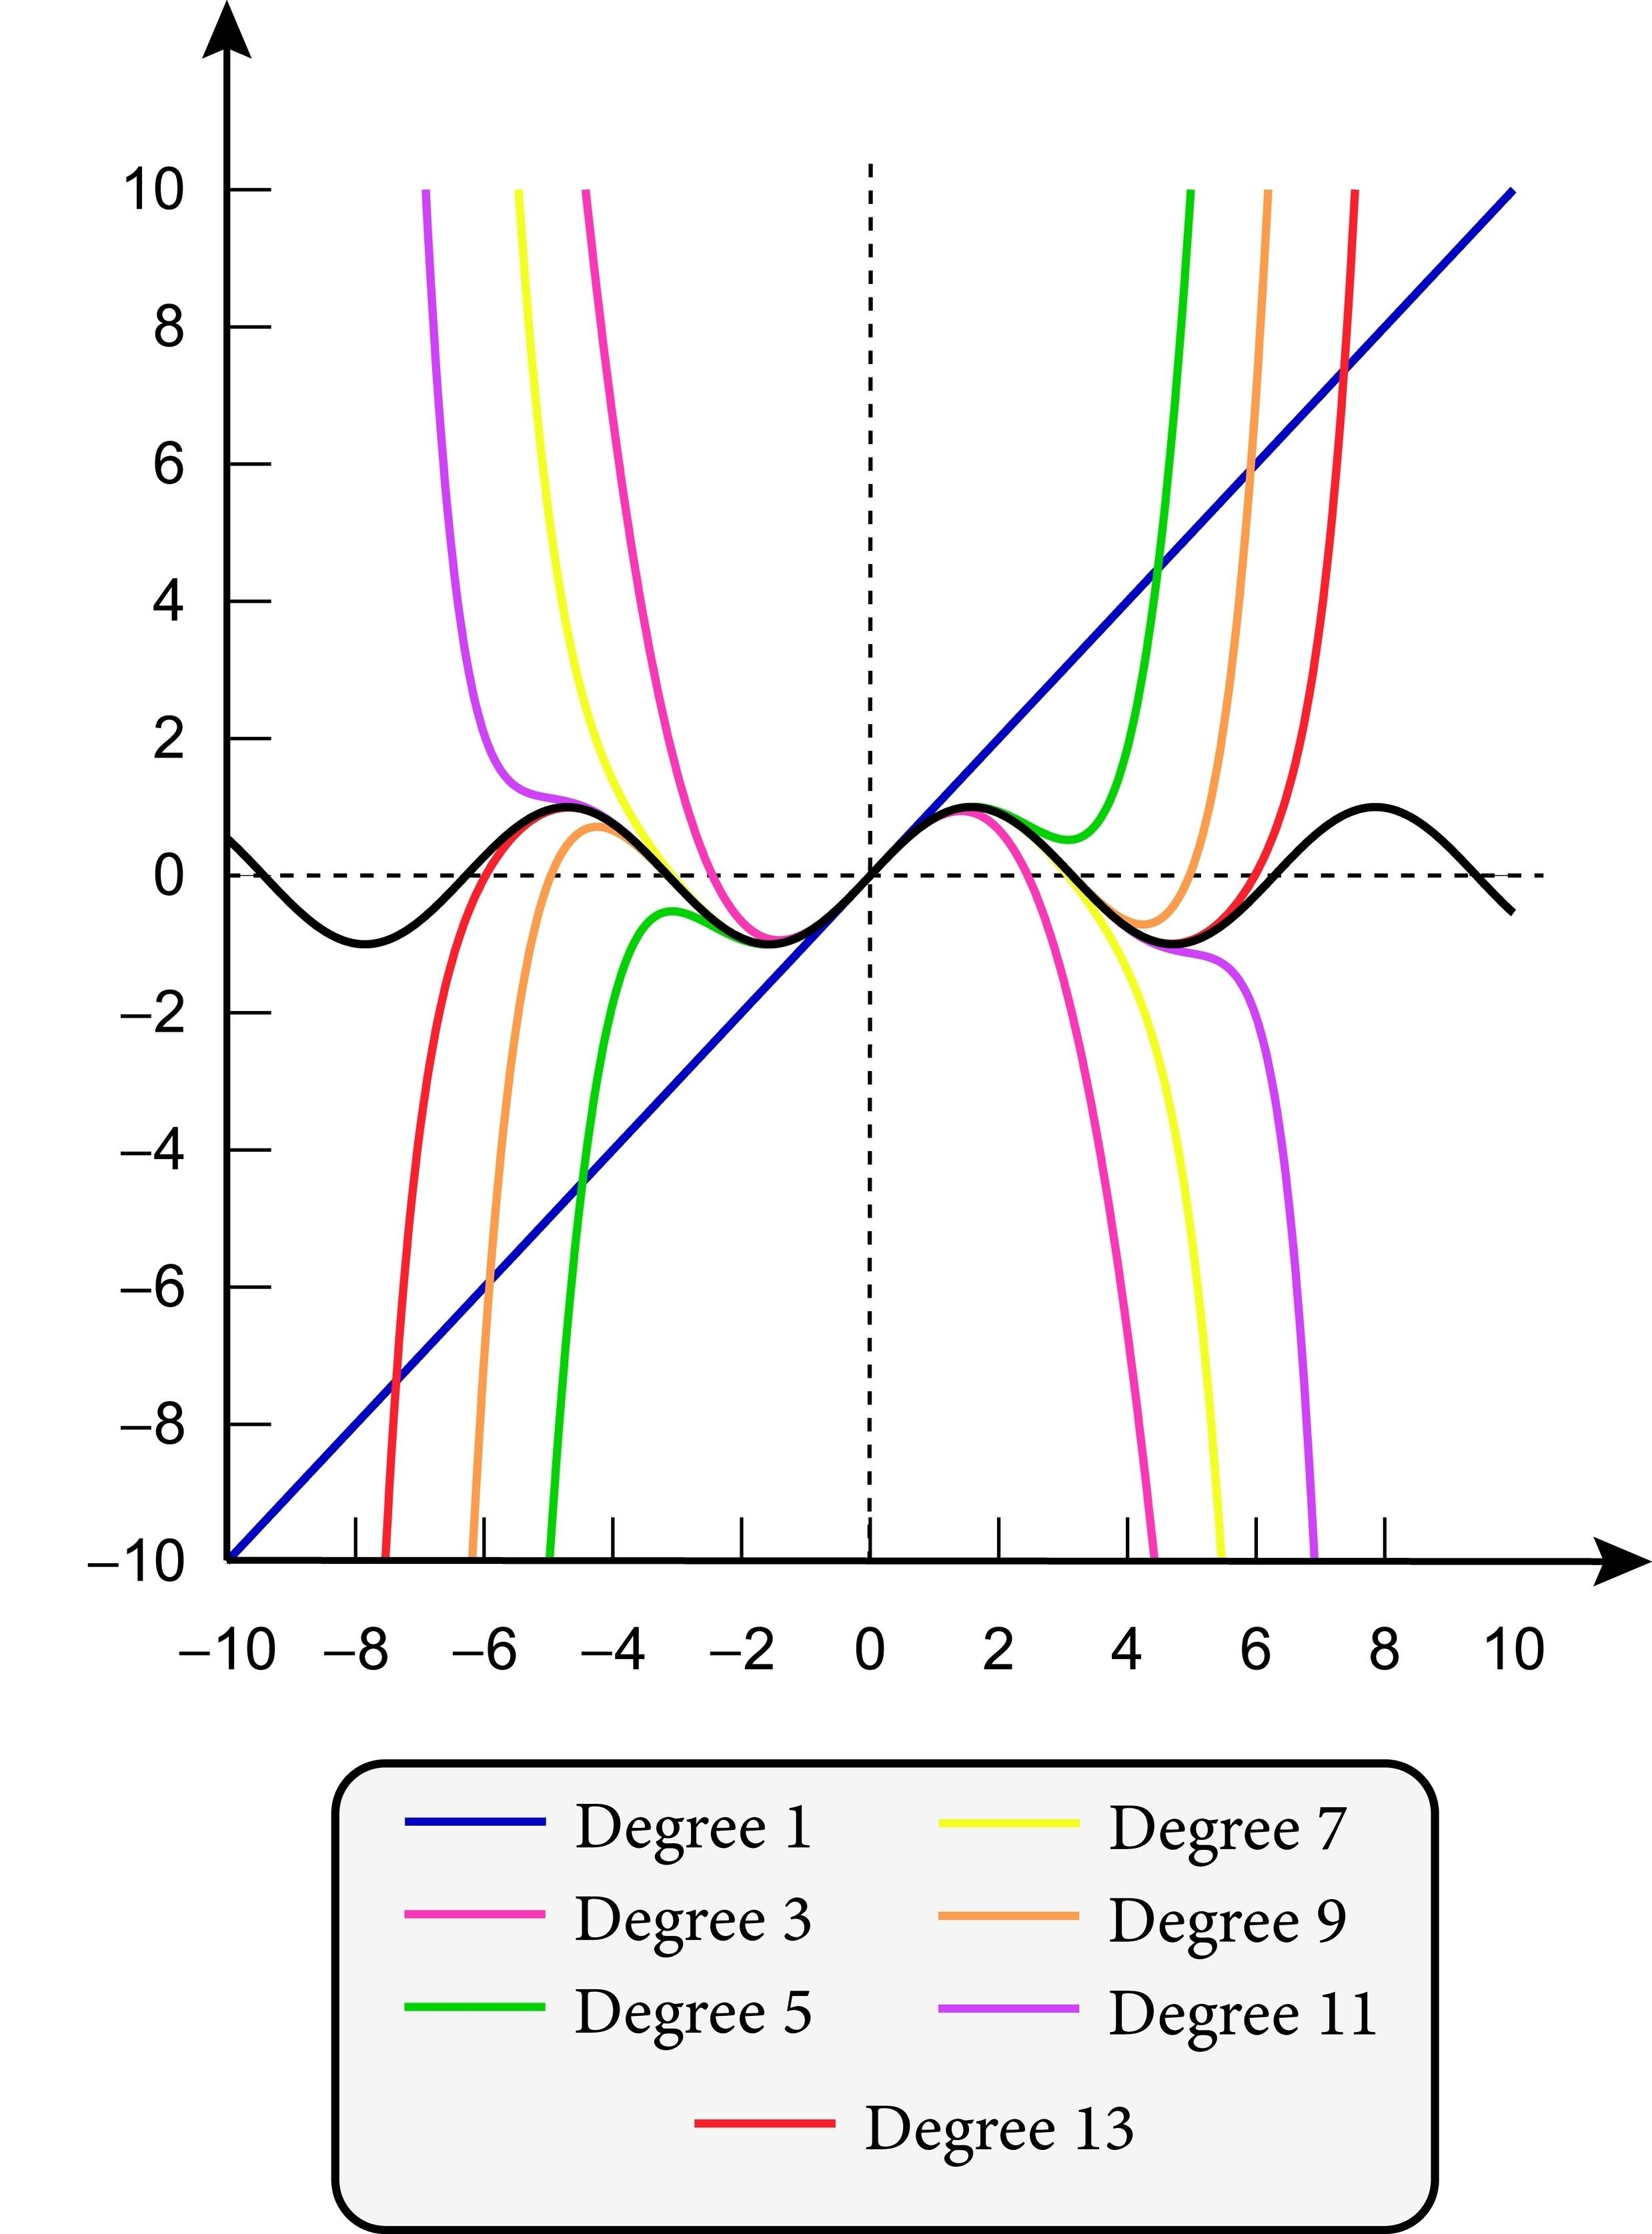
\includegraphics[width=0.98\linewidth,height=0.72\textheight,keepaspectratio]{images/sine_taylor_series.jpg}
  \end{center}
  \vspace{0.15cm}
  \textbf{This is what you guys have been taught or will be taught in high school calculus classes!}
  \vspace{0.3cm}
\end{frame}

% Slide 10: Implementation in Java
\begin{frame}[fragile]{Implementation in Java}
  The mathematical summation is translated into a \texttt{for} loop.
  \begin{block}{Java Logic}
\begin{verbatim}
double x = 1.0; 
double result = 0;

for (int i = 0; i < 5; i++) {
  double term = Math.pow(x, 2*i + 1) / factorial(2*i + 1);
  if (i % 2 == 0) {
    result += term;
  } else {
    result -= term;
  }
}
\end{verbatim}
  \end{block}
\end{frame}

% Slide 11: Implementation in Python
\begin{frame}[fragile]{Implementation in Python}
  The mathematical summation is translated into a \texttt{for} loop.
  \begin{block}{Python Logic}
\begin{verbatim}
x = 1.0
result = 0
for i in range(5):
  term = x**(2*i + 1) / factorial(2*i + 1)
  if i % 2 == 0:
    result += term
  else:
    result -= term
\end{verbatim}
  \end{block}
\end{frame}







% Slide 13: Real-world uses of transcendentals and linear algebra
\begin{frame}{Why This Math Matters: Trig, \texorpdfstring{$\exp$}{exp}, and Linear Algebra}
  \begin{itemize}
    \item \textbf{Games and engines (e.g.\ Unity):} Rotations, camera/view transforms, and animation use trig everywhere; lighting and motion often combine trig with linear algebra (vectors, matrices).
    \item \textbf{Physics simulation:} Springs, waves, and oscillations use $\sin$ and $\cos$; damping, growth, and half-lives use $\exp$ (exponential decay and continuous-time models).
    \item \textbf{AI and machine learning:} Networks are built from matrix multiplies and linear algebra; softmax and many probabilistic models use $\exp$; classical ML (e.g.\ \textbf{linear regression}) is explicit linear algebra on data matrices.
    \item \textbf{Shared theme:} Transcendental functions and linear systems are how we turn continuous models into code that runs at finite precision---the same bridge as Taylor series for $\sin(x)$.
  \end{itemize}
\end{frame}

% Slide 14: Comparison and conclusion
\begin{frame}{Validation of Results}
  The approximation is compared against the standard library:
  \begin{itemize}
    \item \textbf{Taylor Approximation (5 terms):} 0.84147101...
    \item \textbf{Java Math.sin(1):} 0.84147098...
    \item \textbf{Python math.sin(1):} 0.84147098...
  \end{itemize}
  \vspace{0.5cm}
  \begin{alertblock}{Conclusion}
    Mathematical abstraction is bridged by software loops. This logic serves as the foundation for modern computational tools.
  \end{alertblock}
\end{frame}




\end{document}












